\documentclass[times, 12pt]{article}
\usepackage{times}

\usepackage{amsmath, amsfonts, amssymb}                 % Packages to allow inclusion of graphics
\usepackage{graphics}                 % Packages to allow inclusion of graphics
\usepackage{hyperref}                 % For creating hyperlinks in cross references
\usepackage{listings}                 % Source code listing

    \addtolength{\oddsidemargin}{-.875in}
    \addtolength{\evensidemargin}{-.875in}
    \addtolength{\textwidth}{1.75in}

%    \addtolength{\Tmargin}{-.875in}
%    \addtolength{\textheight}{1.75in}

\title{Hardware LU-Decomposition \\ Using Field Programmable Gate Arrays}
\author{Matthew Bennett \quad \today }
 \date{ }

\begin{document}
\pagestyle{plain} \maketitle

\begin{abstract}
$LU$-decomposition is an operation to factor an $n \times n$ square
matrix $A$ in to the product of a lower triangular matrix $L$ and an
upper triangular matrix $U$ so that $A = LU$. The algorithm precedes
many other numerical algorithms--for instance finding the inverse of
a nonsingular matrix, or solving a linear system--so it is useful to
optimize this operation in hardware. The performance of an FPGA
factorization is obtained and compared with a serial soft processor.
\end{abstract}

\newpage

\section*{Background}

Many problems in computer science can be reduced to solving large
systems numerically. For example, in information retrieval, the
Hypertext Induced Topics Search algorithm for page ranking
\cite{kleinberg} can be modeled as a graph connectivity problem,
which is in turn isomorphic to the problem of matrix multiplication
of two square matrices. The problem of matrix multiplication has an
algorithmic complexity of $\Theta \left( n^3 \right)$. However, in
information retrieval, the graph may be as large as the number of
pages on the internet ($n \approx 10^{9}$). Luckily, matrix
algorithms are often highly independent, making them distributable
over many processing elements. One way to deal with this complexity
is to use a traditional multiprocessing machine, or a cluster, to
run the independent parts in parallel \cite{bennett}. Another method
is to encode in hardware the operations needed. This article
investigates the feasibility of implementing such a scheme for $LU$
factorization of a square matrix over the field of rationals.

\section*{Approach}

A hardware design technique known as compile-time polymorphism is
used to achieve a hardware design that is flexible enough to
represent and process a matrix of any size, and yet abstract enough
to be easily comprehensible. For example, a universal piece of
hardware called `square matrix' can be defined to represent a $1
\times 1$ square matrix. Another hardware unit with the same name
can then be defined connecting four `square matrix' types together.
These do not have to be the $1 \times 1$ basic type, but can also be
the abstracted type which is recursively defined. In this way, the
compiler can produce a circuit for whatever size of square matrix is
needed, before placing the circuit on the chip. A similar process is
used to specify invariant structure inherent in the algorithm, since
many matrix algorithms are defined in terms of submatrix algorithms
(e.g. Cramer's Rule). Sudarsanam \cite{sudar} uses polymorphism
instead for processing the data at a variable clock rate, but these
approaches should produce a similar result. The FPGA itself can be
seen as a passive substrate in which logic circuits can be defined
and reconfigured at any time, but the general idea is beyond the
scope of this article.

\section*{Test Platform}

The serial test-bed was a single-core Pentium 4 1.2 Ghz. The C++
code used is a presumed near-optimal.

The FPGA platform used was a Spartan-3 board, operating at 26 Mhz.

\section*{Results}

It is very easy to provide results for powers of two, using
polymorphism (all units decompose into two units at every level), so
matrices of size 4, 8, 16, 32, 64, 128, and 256 were used. During
some trials, the matrices of size 256 by 256 would not fit into the
Spartan, but worked in the simulator, so those results were
extrapolated and are only shown for emphasis. The curve fitted is
quadratic, so complexity could be quadratic due to the way the
compiler handles the decomposition.

\begin{figure}
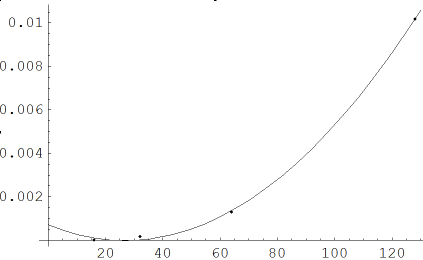
\includegraphics{lin_final1.png}
\caption{26 Mhz FPGA Computation time as a function of N, Size of
Decomposition Matrix}
\end{figure}

The serial (control) code was implemented as Doolittle's algorithm
as described in Wikipedia \cite{wiki}, and is comprised of less than
one page of C++. I found that this method was not optimal for large
matrices, compared to the results obtained from a third party. I
found multiple copies of this code across the web, attributed to
different authors. \cite{code}

\begin{figure}
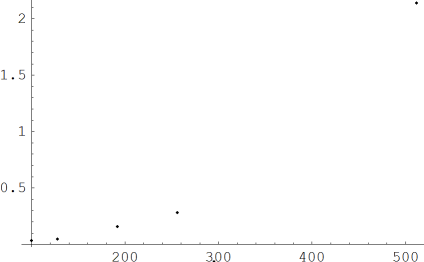
\includegraphics{lin_final2.png}
\caption{1.2 Ghz P4 using an optimized BLAS algorithm in C}
\end{figure}

Its obvious that there are serious flaws in the data collected
(differences in size, etc), but there were serious technical
challenges in collecting good data. Large matrices would not fit
into the tiny memory of the Spartan FPGA, and very small matrices
ran too fast on the benchmark PC to get accurate timing results.
This is why the graphs / data plots of the two systems to not
coincide on N, the number of rows / columns in the square matrix.
Still, we can see that the benchmark system blows up when n=512 or
so, so the FPGA might be able to outperform it if it could only hold
a matrix of that size.

Clearly, the serial code performs better on a modern traditional PC
than the FPGA for small N. This is due to higher level of
abstraction supported by a fast clock and a well-designed supporting
code base. The inherent parallelism of the FPGA produces a gain in
the long run, somewhere around $n=512$.

\section*{Future Work}

The methodology will be improved to provide more meaningful, more
conclusive results. Other algorithms may also be investigated for
various other matrix related computations which are highly
independent.

A more extensive treatment of this topic can be found in Wang and
Ziavras \cite{wang}.

\begin{thebibliography}{9}

\bibitem{kleinberg} Kleinberg, J. {\bf Authoritative Sources in a Hyperlinked Environment.} Journal~of~the~ACM, Vol. 46, No. 5, September 1999, pp. 604�--632.

\bibitem{bennett} Bennett, M. Stone, S. Zhang, C. {\bf A Scalable Parallel HITS Algorithm for Page Ranking} Symposium of High Performance Computing Technology and
Applications (HPCTA|06, IMSCCS|06). June 2006: Hangzhou.

\bibitem{sudar} Sudarsanam, A. Aravind, D.
{\bf Implementation of Polymorphic Matrix Inversion using Viva}
Retrieved from
http://www.klabs.org/mapld05/presento/171\_sudarsanam\_p.ppt on July
24, 2006.

\bibitem{wiki} Wikipedia: LU Decomposition. Retrieved from
http://en.wikipedia.org/wiki/LU\_decomposition on July 26, 2006.

\bibitem{wang} Wang, X. and Ziavras, S. {\bf Parallel LU Factorization of Sparse Matrices on FPGA-Based Configurable Computing Engines} Retrieved from
http://web.njit.edu/~ziavras/CCPE-2003.PDF July 26, 2006.

\bibitem{code} Retrieved from http://comp.cs.ehime-u.ac.jp/~ogata/nac/le\_ludecomp\_cpp.tgz . Original author unknown.

\end{thebibliography}

\end{document}
